\section{Software Design}

\subsection{Global Function parameterize()}

This package's entry point is:

\begin{ccExampleCode}

// Compute a 1 to 1 mapping from a triangular 3D surface 'mesh' to 2D circle,
// using Floater Mean Value Coordinates algorithm.
// 1 to 1 mapping is guaranteed.
template <class ParameterizationMesh_3>
typename Parameterizer_traits_3<ParameterizationMesh_3>::Error_code
parameterize(ParameterizationMesh_3* mesh)
{
    Mean_value_coordinates_parameterizer_3<ParameterizationMesh_3> parameterizer;
    return parameterizer.parameterize(mesh);
}

// Compute a 1 to 1 mapping from a triangular 3D surface 'mesh'
// to a piece of the 2D space.
// 1 to 1 mapping may be guaranteed or not, depending of
// ParameterizerTraits_3 algorithm chosen.
template <class ParameterizationMesh_3, class ParameterizerTraits_3>
typename Parameterizer_traits_3<ParameterizationMesh_3>::Error_code
parameterize(ParameterizationMesh_3* mesh,
             ParameterizerTraits_3 parameterizer)
{
    return parameterizer.parameterize(mesh);
}

\end{ccExampleCode}

You may notice that these global functions simply call the
parameterize() method of a \ccc{ParameterizerTraits_3} object.
The purpose of these global functions is:
\begin{itemize}
\item to be consistent with other CGAL algorithms that are also provided as
      global functions, e.g. \ccc{convex_hull_2}()
\item to provide a default parameterization method (Floater Mean Value Coordinates),
      which wouldn't be possible with a direct call to an object's method
\end{itemize}

You may also wonder why there is not just one parameterize() function with a
default \ccc{ParameterizerTraits_3} argument equal to
\ccc{Mean_value_coordinates_parameterizer_3<ParameterizationMesh_3>}.
The reason is simply that this is not allowed by the C++ standard (see
\cite{cgal:ansi-is14882-98}, paragraph 14.1/9).


\subsection{ParameterizerTraits\_3 is not really a Traits Class}

\ccc{ParameterizerTraits_3} models modify the behavior of the global function
\ccc{parameterize}() - hence the {\em Traits} in the name.
On the other hand, \ccc{ParameterizerTraits_3} models do not modify the behavior
of a common parameterization algorithm - as you might expect.

In this package, we focus on triangulated surfaces that are homeomorphic to a
disk and on piecewise linear mappings into a planar domain.
A consequence is that the skeleton of all parameterization methods of this
package is the same:
\begin{itemize}
\item Allocate a sparse linear system A*X = B
\item Parameterize the mesh border and initialize B
\item Parameterize the inner points of the mesh and set A coefficients
\item Solve the system
\end{itemize}

It is tempting to make the parameterization method a traits class that
modifies the behavior of a common parameterization algorithm.

On the other hand, there are several differences among methods:
\begin{itemize}
\item Fixed border methods need to parameterize all border vertices,
      when free border methods parameterize only two vertices
\item Some methods create symmetric definite positive systems,
      which may be solved more efficiently than general systems
\item Most parameterization methods use two \#vertices x \#vertices systems,
      when Least Squares Conformal Maps uses one (2 * \#triangles) x \#vertices system
\item Most parameterization methods invert the A matrix,
      when Least Squares Conformal Maps solves the system in the least squares sense.
\end{itemize}

Eventually, the software design chosen is:
\begin{itemize}
\item Each \ccc{ParameterizerTraits_3} model implements its own version
      of the parameterization algorithm as a parameterize() method
\item Each \ccc{ParameterizerTraits_3} model has template arguments
      defining the border parameterization and sparse linear solver to use,
      with default values adapted to the method
\item Code factorization is achieved using a class hierarchy and (few) virtual methods.
\end{itemize}

% Include parameterizer_class_diagram.png/eps figure
\begin{figure}[bht]
    \begin{center}
        % Image
        \begin{ccTexOnly}
            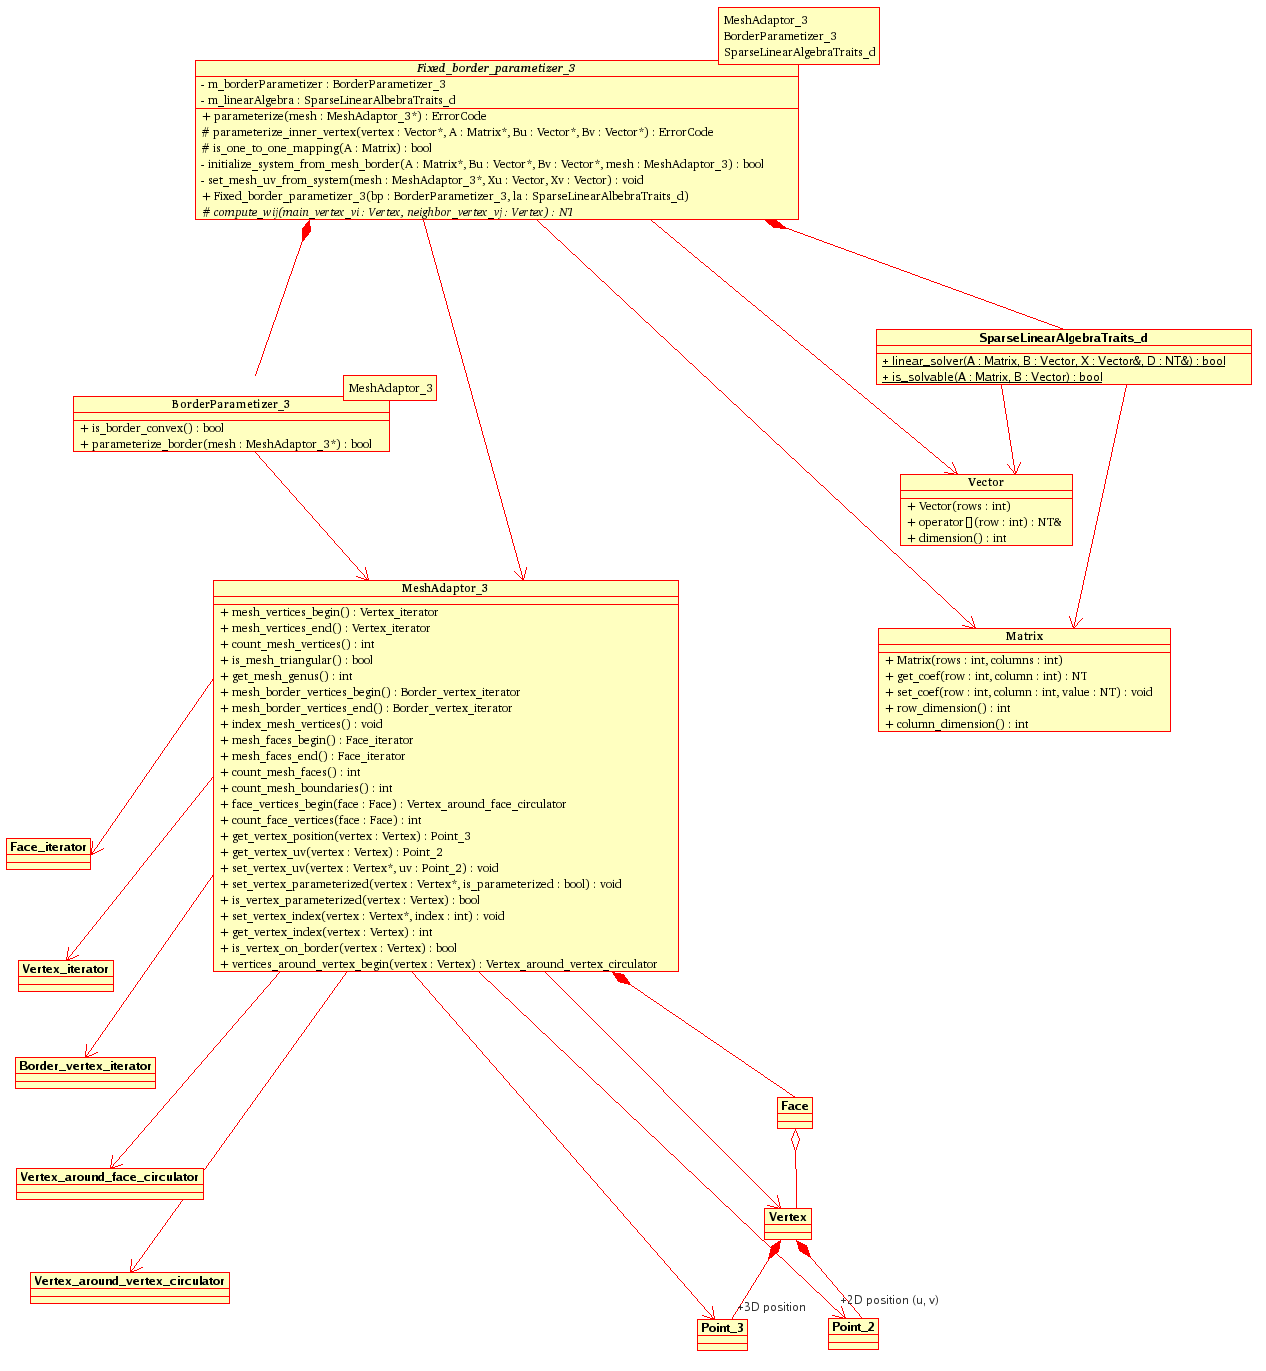
\includegraphics{Parameterization/parameterizer_class_diagram}
        \end{ccTexOnly}
        \begin{ccHtmlOnly}
            <img border=0 src="./parameterizer_class_diagram.png" align=center WIDTH="80%">
        \end{ccHtmlOnly}
        \label{parameterization-fig-parameterizer_class_diagram}

        % Title
        \caption{A parameterizer's UML class diagram (main types and methods only)}
    \end{center}
\end{figure}

% Include parameterizers_class_hierarchy.png/eps figure
\begin{figure}[bht]
    \begin{center}
        % Image
        \begin{ccTexOnly}
            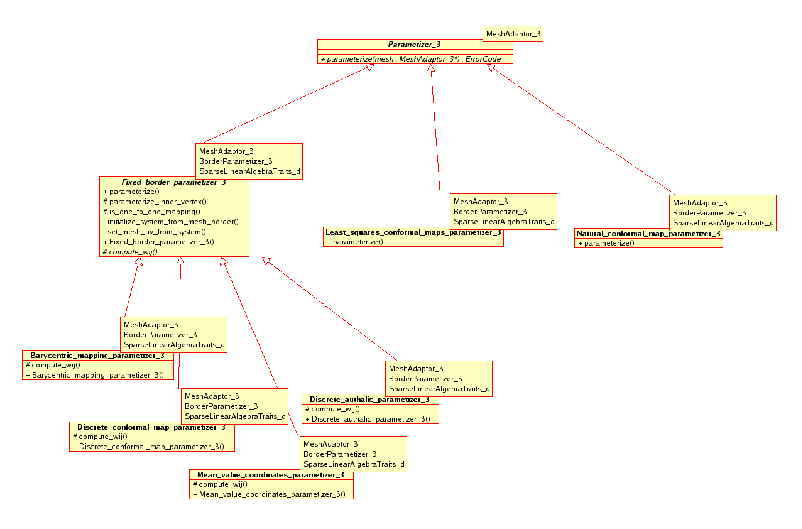
\includegraphics{Parameterization/parameterizers_class_hierarchy}
        \end{ccTexOnly}
        \begin{ccHtmlOnly}
            <img border=0 src="./parameterizers_class_hierarchy.png" align=center WIDTH="80%">
        \end{ccHtmlOnly}
        \label{parameterization-fig-parameterizers_class_hierarchy}

        % Title
        \caption{Parameterizers class hierarchy}
    \end{center}
\end{figure}


\subsection{Fixed\_border\_parameterizer\_3 Class}

Linear fixed border parameterization algorithms are very close. They mainly
differ by the energy that they try to minimize, i.e. by the value of the $w_{ij}$
coefficient of the A matrix, for $v_i$ and $v_j$ neighbor vertices of the mesh
\cite{cgal:fh-survey-05}.

The consequence is that most of the code of the fixed border methods
is factorized in the \ccc{Fixed_border_parameterizer_3} class.
Subclasses:
\begin{itemize}
\item must provide \ccc{BorderParameterizer_3} and \ccc{SparseLinearAlgebraTraits_d} template parameters that make sense
\item must implement \ccc{compute_w_ij}() to compute $w_{ij}$ = (i,j) coefficient of matrix A for $v_j$ neighbor vertex of $v_i$
\item may implement an optimized version of \ccc{is_one_to_one_mapping}()
\end{itemize}

See \ccc{Barycentric_mapping_parameterizer_3} class as an example.


\subsection{Border Parameterizations}

Border Parameterizations are models of the \ccc{BorderParameterizer_3} concept.

To simplify the implementation, \ccc{BorderParameterizer_3} models know only the
\ccc{ParameterizationMesh_3} mesh class. They do not know the parameterization algorithm
nor the sparse linear solver used.


\subsection{MeshAdaptor\_3 and PatchableMeshAdaptor\_3 Concepts}

All parameterization methods are templated by the kind of mesh they are applied on.
The mesh type must be a model of \ccc{ParameterizationMesh_3}.

The purpose of such a model is to:
\begin{enumerate}
\item Support several kind of meshes
\item Hide the implementation of extra fields specific to the parameterization domain
      (\ccc{index}, \ccc{u}, \ccc{v}, \ccc{is_parameterized})
\item Handle in the mesh type the complexity of virtually {\em cutting} a mesh
      to make it homeomorphic to a disk (instead of duplicating this
      code in each parameterization method)
\end{enumerate}

Two options are possible for 1) and 2):
\begin{itemize}
\item Pass to all classes and methods a mesh pointer, a traits class to manipulate it,
      and accessors to the extra fields arrays.
      This is the choice of the Boost Graph Library with \ccc{boost::graph_traits<>}
      and the property maps.
\item Pass to all classes and methods an object that points to the actual mesh and knows
      how to access to it. This is the Adaptor concept \cite{cgal:ghjv-dpero-95}.
\end{itemize}

The current design of this package uses the second option, which is simpler.
Of course, we may decide to switch to the first one to reach a deeper integration
of CGAL with Boost.

Point 3) is solved by class \ccc{Parameterization_mesh_patch_3}, which takes care
of virtually {\em cutting}
a patch in a \ccc{ParameterizationPatchableMesh_3} mesh, to make it appear as a topological disk
with a \ccc{ParameterizationMesh_3} interface.
\ccc{ParameterizationPatchableMesh_3} inherits from concept \ccc{ParameterizationMesh_3} and adds
the ability to support patches and virtual seams.
This mainly means that:
\begin{itemize}
\item vertices can be tagged as inside or outside the patch to parameterize
\item the fields specific to parameterizations (\ccc{index}, \ccc{u}, \ccc{v}, \ccc{is_parameterized})
      can be set per {\em corner} (aka half-edge)
\end{itemize}


\subsection{SparseLinearAlgebraTraits\_d Concept}

This package solves sparse linear systems using solvers which are models
of \ccc{SparseLinearAlgebraTraits_d}.

\ccc{SparseLinearAlgebraTraits_d} is a sub-concept of \ccc{LinearAlgebraTraits_d} concept
in \ccc{Kernel_d}.
The goal is to adapt easily code wriiten for dense matrices to sparse ones,
and vice-versa.


\subsection{Cutting a Mesh}

In this package, we focus on triangulated surfaces that are homeomorphic to a
disk.

Computing a cut that transforms
a closed mesh of arbitrary genus into a topological disk is a research domain
of its own. This package doesn't cover this subject.



